\chapter{Introduction}\label{ch:1}
\lipsum[1-3]

The remaining chapters are organised as described in \cref{ch:2}; \cref{app:A} contains derivations \citep{ch1-1,ch1-2}.

\section{Overview and Motivation}\label{sec:c1s1}
\kant[2-11]

This section builds on the material in \cref{ch:1}, \cref{ch:2} and the prior work of \citet{ch1-3}; see also \citep{ch1-10,ch1-2}.

\begin{equation}\label{eq:c1s1-a}
  I = \int_{0}^{1}\!\!\int_{0}^{1} \frac{\sin(\pi x)\sin(\pi y)}{1+x^2+y^2}\,\mathrm{d}x\,\mathrm{d}y \approx \frac{1}{M}\sum_{m=1}^{M} h(\xi_m),
\end{equation}
with variance decreasing as
\begin{equation}\label{eq:c1s1-b}
  \operatorname{Var}\bigl[\hat I_M\bigr] = \frac{1}{M}\Bigl(\int h^2\,\mathrm{d}\mu - I^2\Bigr) = \mathcal{O}(M^{-1}).
\end{equation}

Equations~\eqref{eq:c1s1-a} and~\eqref{eq:c1s1-b} are used throughout the remainder of this section.

\kant[7-11]

\subsection{Quantitative behaviour}\label{sec:c1s1-q}
Results are collected in \cref{tab:c1s1} and visualised in \cref{fig:c1s1-f1}. Similar trends were reported in~\citep{ch1-5,ch1-12}.

\begin{table}[htbp]
\centering
\caption{Summary of measured quantities for experiment set \texttt{c1s1}.}\label{tab:c1s1}
\begin{tabular}{lrrr}
\toprule
Method & Score & Latency & Error \\
\midrule
Alpha & \num{63.2} & \SI{7.57}{\milli\second} & \num{1.017e-4} \\
Beta & \num{28.2} & \SI{7.17}{\milli\second} & \num{2.830e-1} \\
Gamma & \num{93.3} & \SI{3.21}{\milli\second} & \num{1.179e-5} \\
Delta & \num{1.9} & \SI{9.30}{\milli\second} & \num{4.050e-2} \\
Epsilon & \num{44.2} & \SI{7.21}{\milli\second} & \num{5.221e-4} \\
\bottomrule
\end{tabular}
\end{table}

\begin{figure}[htbp]
\centering
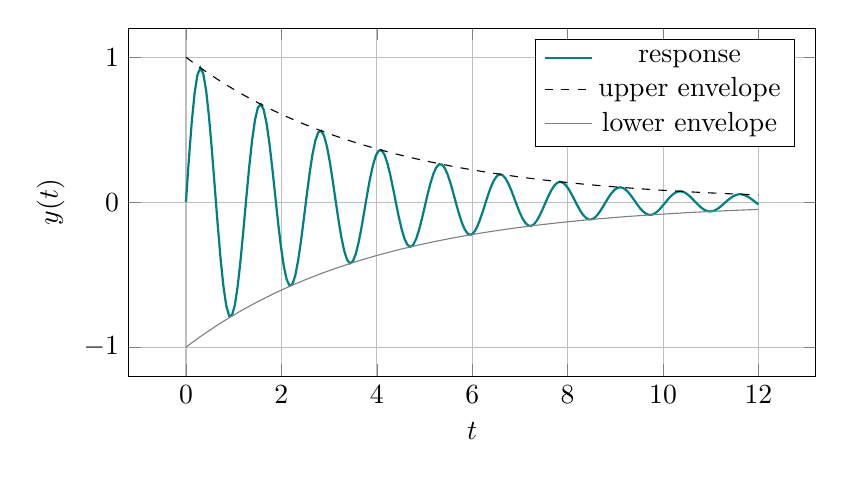
\begin{tikzpicture}\begin{axis}[width=0.85\linewidth,height=6cm,xlabel={$t$},ylabel={$y(t)$},legend pos=north east,grid=both,domain=0:12]
\addplot[teal,thick,samples=200]{sin(deg(5*x))*exp(-x/4)};
\addplot[black,dashed,samples=200]{exp(-x/4)};
\addplot[gray,samples=200]{-exp(-x/4)};
\legend{response,upper envelope,lower envelope}
\end{axis}\end{tikzpicture}
\caption{Generated figure for \texttt{c1s1-f1} (parameters $a=5$, $b=4$).}\label{fig:c1s1-f1}
\end{figure}

\kant[8-11]

\subsection{Implementation notes}\label{sec:c1s1-i}
The core routine is shown in \cref{lst:c1s1}; its complexity is $\mathcal{O}(N\log N)$ per iteration~\cite{ch1-8}.

\begin{lstlisting}[language=c,caption={Reference implementation for c1s1.},label={lst:c1s1}]
#include <stdio.h>

/* Compute a dot product of two vectors. */
double dot(const double *a, const double *b, int n) {
    double s = 0.0;
    for (int i = 0; i < n; ++i)
        s += a[i] * b[i];
    return s;
}
\end{lstlisting}

\lipsum[6-6]
\begin{theorem}\label{thm:c1s1}
Let $A\in\mathbb{R}^{n\times n}$ be symmetric positive definite with condition number $\kappa$. Then the iteration converges and
$\lVert e_k\rVert_A \le 2\bigl(\tfrac{\sqrt\kappa-1}{\sqrt\kappa+1}\bigr)^k\lVert e_0\rVert_A$.
\end{theorem}
\begin{enumerate}[label=(\roman*)]
\item the bound in \cref{thm:c1s1} is sharp for some initial errors;
\item the constant $2$ cannot be improved in general;
\item preconditioning reduces the effective $\kappa$.
\end{enumerate}

\begin{figure}[htbp]
\centering
\includegraphics[width=0.45\linewidth]{grad1.png}
\caption{Raster/vector asset \texttt{grad1.png} included from the figures directory.}\label{fig:c1s1-i0}
\end{figure}

\begin{figure}[htbp]
\centering
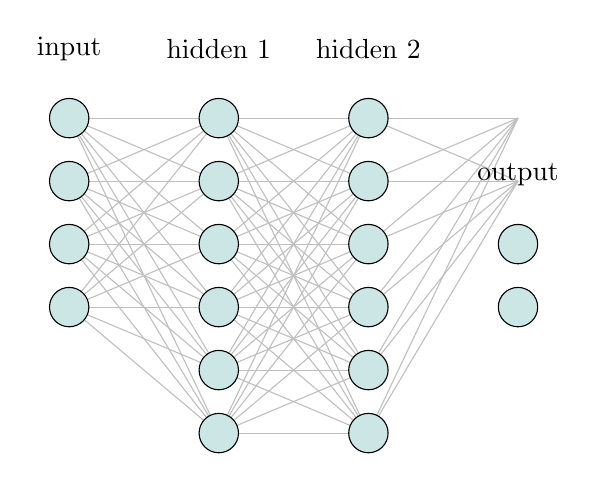
\begin{tikzpicture}[x=1.9cm,y=0.8cm,neuron/.style={circle,draw,fill=teal!20,minimum size=5mm,inner sep=0}]
\foreach \i in {1,...,4}{\foreach \j in {1,...,6}{\draw[gray!50](0,-\i)--(1,-\j);}}
\foreach \i in {1,...,6}{\foreach \j in {1,...,6}{\draw[gray!50](1,-\i)--(2,-\j);}}
\foreach \i in {1,...,6}{\foreach \j in {1,...,2}{\draw[gray!50](2,-\i)--(3,-\j);}}
\foreach \i in {1,...,4}\node[neuron](i\i)at(0,-\i){};
\foreach \i in {1,...,6}\node[neuron](h\i)at(1,-\i){};
\foreach \i in {1,...,6}\node[neuron](g\i)at(2,-\i){};
\foreach \i in {1,...,2}\node[neuron](o\i)at(3,-\i-2){};
\node at(0,0.1){input};\node at(1,0.1){hidden 1};\node at(2,0.1){hidden 2};\node at(3,-1.9){output};
\end{tikzpicture}
\caption{Generated figure for \texttt{c1s1-f2} (parameters $a=2$, $b=4$).}\label{fig:c1s1-f2}
\end{figure}

\kant[9-11]

\section{Mathematical Framework}\label{sec:c1s2}
\lipsum[9-9]

This section builds on the material in \cref{sec:c1s1}, \cref{ch:2} and the prior work of \citet{ch1-9}; see also \citep{ch1-11,ch1-4}.

\begin{equation}\label{eq:c1s2-a}
  I = \int_{0}^{1}\!\!\int_{0}^{1} \frac{\sin(\pi x)\sin(\pi y)}{1+x^2+y^2}\,\mathrm{d}x\,\mathrm{d}y \approx \frac{1}{M}\sum_{m=1}^{M} h(\xi_m),
\end{equation}
with variance decreasing as
\begin{equation}\label{eq:c1s2-b}
  \operatorname{Var}\bigl[\hat I_M\bigr] = \frac{1}{M}\Bigl(\int h^2\,\mathrm{d}\mu - I^2\Bigr) = \mathcal{O}(M^{-1}).
\end{equation}

Equations~\eqref{eq:c1s2-a} and~\eqref{eq:c1s2-b} are used throughout the remainder of this section.

\lipsum[104-105]

\subsection{Quantitative behaviour}\label{sec:c1s2-q}
Results are collected in \cref{tab:c1s2} and visualised in \cref{fig:c1s2-f1}. Similar trends were reported in~\citep{ch1-5,ch1-13}.

\begin{table}[htbp]
\centering
\caption{Summary of measured quantities for experiment set \texttt{c1s2}.}\label{tab:c1s2}
\begin{tabular}{lrrr}
\toprule
Method & Score & Latency & Error \\
\midrule
Alpha & \num{18.7} & \SI{3.70}{\milli\second} & \num{8.062e-3} \\
Beta & \num{9.8} & \SI{4.40}{\milli\second} & \num{5.067e-2} \\
Gamma & \num{54.3} & \SI{8.33}{\milli\second} & \num{3.964e-1} \\
Delta & \num{49.0} & \SI{0.53}{\milli\second} & \num{6.627e-5} \\
Epsilon & \num{61.7} & \SI{5.77}{\milli\second} & \num{6.177e-2} \\
\bottomrule
\end{tabular}
\end{table}

\begin{figure}[htbp]
\centering
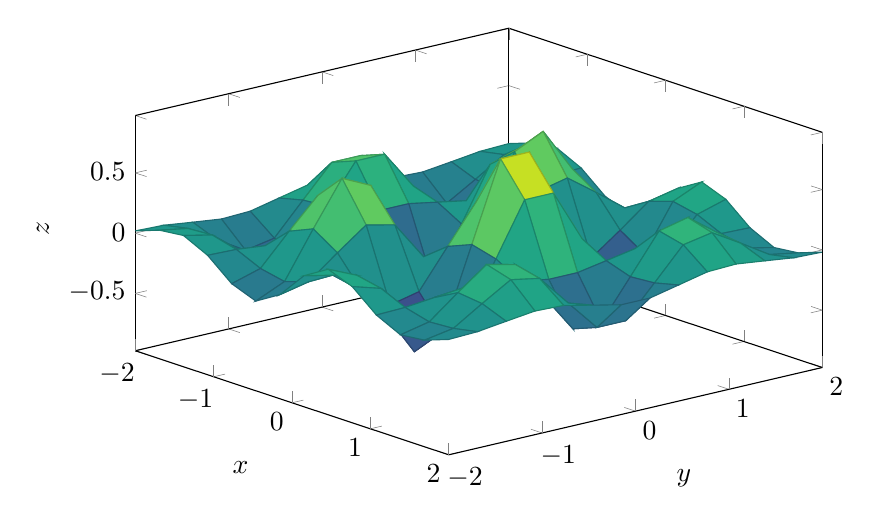
\begin{tikzpicture}\begin{axis}[width=0.85\linewidth,height=7cm,view={50}{30},colormap/viridis,xlabel=$x$,ylabel=$y$,zlabel=$z$]
\addplot3[surf,samples=14,domain=-2:2]{sin(deg(3*x))*cos(deg(3*y))*exp(-(x^2+y^2)/3)};
\end{axis}\end{tikzpicture}
\caption{Generated figure for \texttt{c1s2-f1} (parameters $a=3$, $b=3$).}\label{fig:c1s2-f1}
\end{figure}

\kant[9-10]

\subsection{Implementation notes}\label{sec:c1s2-i}
The core routine is shown in \cref{lst:c1s2}; its complexity is $\mathcal{O}(N\log N)$ per iteration~\cite{ch1-8}.

\begin{lstlisting}[language=python,caption={Reference implementation for c1s2.},label={lst:c1s2}]
def conjugate_gradient(A, b, tol=1e-8, maxit=500):
    x = b * 0
    r = b - A @ x
    p = r.copy()
    for k in range(maxit):
        Ap = A @ p
        alpha = (r @ r) / (p @ Ap)
        x += alpha * p
        r_new = r - alpha * Ap
        if (r_new @ r_new) ** 0.5 < tol:
            break
        p = r_new + ((r_new @ r_new) / (r @ r)) * p
        r = r_new
    return x
\end{lstlisting}

\lipsum[104-104]
\begin{theorem}\label{thm:c1s2}
Let $A\in\mathbb{R}^{n\times n}$ be symmetric positive definite with condition number $\kappa$. Then the iteration converges and
$\lVert e_k\rVert_A \le 2\bigl(\tfrac{\sqrt\kappa-1}{\sqrt\kappa+1}\bigr)^k\lVert e_0\rVert_A$.
\end{theorem}
\begin{enumerate}[label=(\roman*)]
\item the bound in \cref{thm:c1s2} is sharp for some initial errors;
\item the constant $2$ cannot be improved in general;
\item preconditioning reduces the effective $\kappa$.
\end{enumerate}

\begin{figure}[htbp]
\centering
\includegraphics[width=0.45\linewidth]{rings.png}
\caption{Raster/vector asset \texttt{rings.png} included from the figures directory.}\label{fig:c1s2-i0}
\end{figure}

\lipsum[91-91]

\section{Analysis and Validation}\label{sec:c1s3}
\lipsum[53-53]

This section builds on the material in \cref{sec:c1s2}, \cref{ch:2} and the prior work of \citet{ch1-5}; see also \citep{ch1-11,ch1-9}.

\begin{equation}\label{eq:c1s3-a}
  \hat{\theta} = \arg\min_{\theta\in\Theta}\; \frac{1}{n}\sum_{i=1}^{n}\ell\bigl(y_i, g_\theta(x_i)\bigr) + \lambda\lVert\theta\rVert_2^2 .
\end{equation}
Under standard regularity conditions the estimator is consistent, and its error satisfies
\begin{equation}\label{eq:c1s3-b}
  \mathbb{E}\lVert\hat\theta-\theta^\star\rVert^2 \le \frac{C\,\sigma^2 d}{n} + \lambda^2\lVert\theta^\star\rVert^2 .
\end{equation}

Equations~\eqref{eq:c1s3-a} and~\eqref{eq:c1s3-b} are used throughout the remainder of this section.

\lipsum[15-16]

\subsection{Quantitative behaviour}\label{sec:c1s3-q}
Results are collected in \cref{tab:c1s3} and visualised in \cref{fig:c1s3-f1}. Similar trends were reported in~\citep{ch1-10,ch1-1}.

\begin{table}[htbp]
\centering
\caption{Summary of measured quantities for experiment set \texttt{c1s3}.}\label{tab:c1s3}
\begin{tabular}{lrrr}
\toprule
Method & Score & Latency & Error \\
\midrule
Alpha & \num{38.3} & \SI{5.69}{\milli\second} & \num{2.599e-5} \\
Beta & \num{43.3} & \SI{4.85}{\milli\second} & \num{3.854e-3} \\
Gamma & \num{1.1} & \SI{5.38}{\milli\second} & \num{5.988e-5} \\
Delta & \num{34.9} & \SI{4.59}{\milli\second} & \num{1.224e-2} \\
Epsilon & \num{66.0} & \SI{1.84}{\milli\second} & \num{5.676e-1} \\
\bottomrule
\end{tabular}
\end{table}

\begin{figure}[htbp]
\centering
\begin{tikzpicture}[node distance=9mm and 8mm,>=Stealth,blk/.style={draw,rounded corners,fill=blue!12,minimum width=2.1cm,minimum height=8mm,align=center}]
\node[blk](a){Data\\acquisition};\node[blk,right=of a](b){Pre-\\processing};\node[blk,right=of b](c){Model\\fitting};\node[blk,right=of c](d){Validation};
\node[blk,below=of b](e){Feature\\store};\node[blk,below=of c](f){Parameter\\search};
\draw[->](a)--(b);\draw[->](b)--(c);\draw[->](c)--(d);\draw[->](b)--(e);\draw[->](e)--(f);\draw[->](f)--(c);\draw[->,dashed](d.north)--++(0,.8)-|(a.north);
\begin{scope}[on background layer]\node[draw,dashed,fit=(a)(b)(c)(d)(e)(f),inner sep=6pt,fill=gray!5]{};\end{scope}
\end{tikzpicture}
\caption{Generated figure for \texttt{c1s3-f1} (parameters $a=4$, $b=3$).}\label{fig:c1s3-f1}
\end{figure}

\kant[8-10]

\subsection{Implementation notes}\label{sec:c1s3-i}
The core routine is shown in \cref{lst:c1s3}; its complexity is $\mathcal{O}(N\log N)$ per iteration~\cite{ch1-7}.

\begin{lstlisting}[language=python,caption={Reference implementation for c1s3.},label={lst:c1s3}]
def conjugate_gradient(A, b, tol=1e-8, maxit=500):
    x = b * 0
    r = b - A @ x
    p = r.copy()
    for k in range(maxit):
        Ap = A @ p
        alpha = (r @ r) / (p @ Ap)
        x += alpha * p
        r_new = r - alpha * Ap
        if (r_new @ r_new) ** 0.5 < tol:
            break
        p = r_new + ((r_new @ r_new) / (r @ r)) * p
        r = r_new
    return x
\end{lstlisting}

\lipsum[72-72]
\begin{theorem}\label{thm:c1s3}
Let $A\in\mathbb{R}^{n\times n}$ be symmetric positive definite with condition number $\kappa$. Then the iteration converges and
$\lVert e_k\rVert_A \le 2\bigl(\tfrac{\sqrt\kappa-1}{\sqrt\kappa+1}\bigr)^k\lVert e_0\rVert_A$.
\end{theorem}
\begin{enumerate}[label=(\roman*)]
\item the bound in \cref{thm:c1s3} is sharp for some initial errors;
\item the constant $2$ cannot be improved in general;
\item preconditioning reduces the effective $\kappa$.
\end{enumerate}

\kant[3-11]

\unitbib{Chapters/refs-ch1}
